\documentclass[10pt,twocolumn,letterpaper]{article}
\usepackage[review]{cvpr}
\usepackage{graphicx,amsmath,amssymb,booktabs,microtype}
\definecolor{oursteal}{HTML}{008C88}
\definecolor{cvprblue}{rgb}{0.21,0.49,0.74}
\usepackage[pagebackref,breaklinks,colorlinks,allcolors=cvprblue]{hyperref}
\def\confName{CVPR}\def\confYear{2027}
\title{Compositional Neural Mechanics for Physical Prediction Beyond Visual Agreement}
\author{Anonymous submission}
\newcommand{\R}{\mathbb{R}}
\begin{document}
\maketitle
\begin{abstract}
A deformable digital twin should predict what an object will do under a new interaction, not only reproduce its observed images. These objectives differ: under displacement control, scaling material and attachment stiffness together can preserve every rendered view while changing reaction forces. We study a compositional representation that separates a shared neural bulk energy, compliant attachments, explicit contact and body loads, and material-attached Gaussian appearance. Compact energy decoders are pretrained on constitutive responses and frozen; scene adaptation estimates physical descriptors from observed positions. A conventional finite-element solver then predicts deformation and reactions under new commands or initial conditions. Controlled synthetic experiments test three distinct questions: transfer with known descriptors, refinement with unknown descriptors, and dynamic forecasting with shared initial appearance. On six withheld-composition objects, shared laws achieve 0.018\,mm coordinate RMSE, versus 3.089\,mm for a custom supervised direct predictor. An additional stretch observation reduces unknown-parameter prediction error from 0.339 to 0.080\,mm, without establishing an adaptive-policy advantage. Across 24 material worlds and six interaction families, motion RMS is 1.97\,mm versus 10.80 and 11.27\,mm for native PhysTwin and Spring-Gaus adaptations; shared-renderer foreground PSNR is 35.61 versus 25.68 and 25.88\,dB. A matched analytic control remains competitive at 1.84\,mm. We report missing forecasts, numerical-reference sensitivity and uncertainty miscalibration explicitly. The results support composition of learned local mechanics for controlled physical prediction; visual agreement alone remains insufficient evidence of physical accuracy.
\end{abstract}

\begin{figure*}[t]
\centering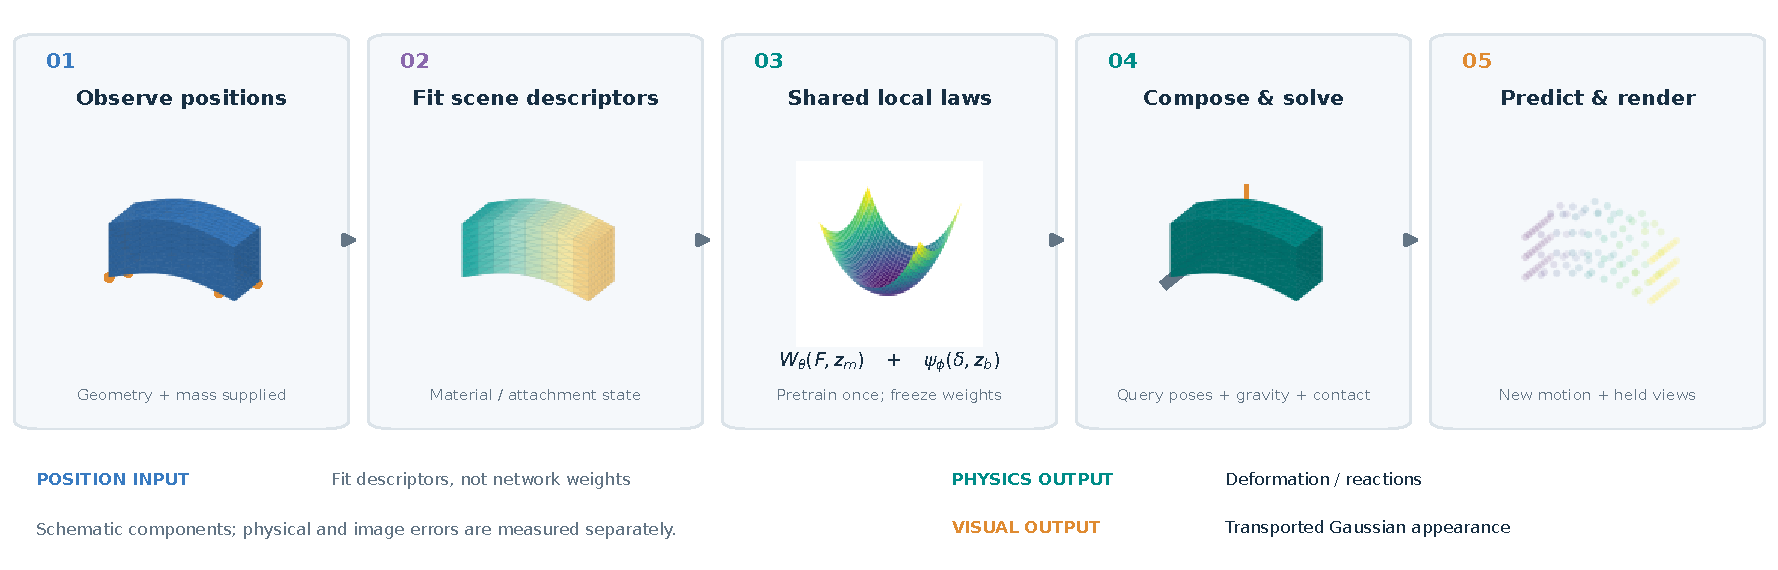
\includegraphics[width=\textwidth]{figures/method_visual.pdf}
\caption{\textbf{Representation and prediction pipeline.} Local constitutive laws are trained once. Scene descriptors are fitted from observed positions with shared weights frozen. Prescribed tool poses, initial conditions, gravity and explicit contact geometry define a query; composed energies produce deformation and reactions through Q2 mechanics. The physical state transports a separately initialized Gaussian appearance model. Geometry and image metrics are evaluated independently on withheld responses. Geometry, mass and observation correspondences are supplied in the present experiments.}
\label{fig:pipeline}
\end{figure*}

\section{Introduction}
Images reveal where a surface is, but not necessarily why it is there. A soft object held between two grippers may deform because its bulk material is compliant, its attachments slip elastically, or both. A reconstruction can therefore render an observed motion convincingly while assigning the wrong response to the next manipulation. For action planning, a matched silhouette does not guarantee correct forces or rebound.

Recent Gaussian and continuum approaches have substantially improved the reconstruction and simulation of deformable scenes~\cite{xie2024physgaussian,zhong2024springgaus,jiang2025phystwin}. Learned constitutive representations also provide a route to sharing material knowledge across scenes~\cite{ma2023nclaw,mittal2025uniphy}. We build on these directions to ask a narrower question: can local learned material and interaction laws be composed into a reusable model whose physical predictions and rendered outputs are evaluated separately?

Our representation associates bulk properties with material coordinates, attachment laws with relations between material and prescribed tools, and collision geometry and gravity with the surrounding scene. Position commands specify how tools move; forces follow from the energy rather than being required as inputs. The physical state drives Gaussian centers and covariances, while appearance parameters remain independent of scene-specific mechanical fitting. This separation permits the same constitutive decoder to be reused across material combinations, geometries and interactions.

The distinction between appearance and mechanics is not merely a matter of metric choice. With no independent body load, multiplying every stiffness-bearing term in a position-controlled equilibrium problem by the same positive constant preserves its equilibrium configurations. Reactions change, but all cameras see the same geometry. Additional views cannot resolve this exact ambiguity. An informative action must change observability, for example through a known gravitational or inertial scale, or measured reactions.

We evaluate these issues through four controlled studies rather than pooling incompatible tasks. First, known-descriptor tests isolate forward transfer of learned local laws. Second, a small inverse problem estimates 15 continuous material and attachment descriptors and measures the benefit of one additional position observation. Third, timed drop experiments compare frozen predictions against native PhysTwin using identical initial Gaussian appearance. Fourth, a six-family benchmark tests changed interactions on 24 independent material worlds against native PhysTwin and Spring-Gaus adaptations, with explicit UniPhy coverage. Stronger compression, impact and bounce examples accompany these studies, while numerical failures remain part of the record.

Our contributions are: (1) a concrete composition of compact conditional bulk and attachment energies with explicit loads, contact and Gaussian transport; (2) a scale-observability analysis connecting image ambiguity to physical response; and (3) a controlled evaluation separating transfer, adaptation, dynamics and appearance, including forecast coverage and reference sensitivity. The individual solver, invariant-energy and Gaussian-transport ingredients are established. Our evidence concerns their composition and the resulting prediction protocol, not a new general-purpose simulator or broad benchmark leadership.



\section{Related Work}
\label{sec:related}

\paragraph{Physical neural scene representations.}
Gaussian splatting provides an explicit, efficiently rendered radiance-field
representation~\cite{kerbl2023gaussians}. Coupling visual representations to
mechanics predates physical Gaussians: PAC-NeRF combines neural radiance fields
with differentiable material point method (MPM) simulation to identify geometry
and physical parameters from calibrated multi-view RGB
video~\cite{li2023pacnerf}. PhysGaussian reconstructs a static Gaussian scene and
generates motion using supplied material and boundary settings; its continuum
deformation map transports Gaussian covariances through the deformation
gradient~\cite{xie2024physgaussian}. Spring-Gaus learns spring-mass dynamics from
multi-view video through staged appearance, geometry and physical
optimization~\cite{zhong2024springgaus}. PhysTwin uses sparse RGB-D interaction
videos, shape priors and lifted image tracks to fit geometry and spring-mass
physics, followed by Gaussian appearance optimization; it demonstrates future
prediction and novel interactions~\cite{jiang2025phystwin}. These works establish
both simulatable visual assets and separation of physical fitting from appearance.

\paragraph{Constitutive reuse and inverse mechanics.}
Learning material response within known governing equations is an established
alternative to learning complete state transitions. NCLaw embeds structured
constitutive networks in differentiable simulation and evaluates transfer across
geometry, initial conditions and boundary conditions~\cite{ma2023nclaw}.
UniPhy learns shared latent-conditioned deformation-gradient projection and
stress networks, pretrained using simulated constitutive supervision; at
inference it freezes their weights and optimizes a material latent against
observed particle trajectories~\cite{mittal2025uniphy}. Thus shared constitutive
representations and scene-specific inverse adaptation already have direct
precedent. Our formulation uses a scalar bulk-energy decoder, derives stress
from that energy, and composes the bulk response with separately parameterized
scene interfaces. The contribution concerns this composition and its evaluated
predictive behavior, rather than priority for constitutive reuse. The elastic
experiments also cover a narrower material class than UniPhy's plastic and
fluid examples.

\paragraph{Generative priors and observed-motion reconstruction.}
PhysDreamer distills video-generation priors into material fields to synthesize
responses to new interactions~\cite{zhang2024physdreamer}. OmniPhysGS uses
text-conditioned diffusion guidance to learn mixtures of constitutive experts
for Gaussian particles~\cite{lin2025omniphysgs}. Their generative supervision
differs from fitting measured motion. PIDG instead uses time-dependent
deformation, predicted velocity and stress, momentum residuals and optical-flow
supervision for monocular dynamic reconstruction~\cite{hong2026pidg}. Its
published formulation does not expose a query-force input. We distinguish
reconstructing observed motion, generating plausible interactions and forecasting
a reset system under changed loading; success on one task does not establish
the others.

\paragraph{Numerics, systems and evaluation.}
DiffPD develops efficient differentiation through implicit projective dynamics,
including contact models and inverse problems~\cite{du2022diffpd}.
i-PhysGaussian couples Gaussian rendering to implicit Newton--GMRES MPM and
evaluates time-step robustness~\cite{cao2026iphysgaussian}. Boba accelerates
PhysTwin-style rollouts through compact spring-mass surrogates and shared-template
batched execution~\cite{pang2026boba}. These contributions motivate separating
material representation from integration, inertia, contact and implementation
effects. Deform360 provides real multi-view visuotactile data and evaluates
per-episode, multi-episode and multi-object prediction~\cite{li2026deform360}.
Our controlled synthetic study uses known geometry and visible three-dimensional
tracks, and compares future motion and Gaussian rendering under matched
observations. It therefore evaluates a specific composed pipeline, with
numerical-reference sensitivity and prediction coverage retained; it does not
establish end-to-end video reconstruction, real-world material identification,
calibrated posterior uncertainty or uncertainty-guided probing.


\section{Compositional Neural Mechanics}
\subsection{State, inputs and outputs}
Let $X\in\Omega_0\subset\R^3$ denote a material coordinate and $x(X,t)=X+u(X,t)$ its current position. Its deformation gradient is $F=\partial x/\partial X$. A scene has a material descriptor field $z_m(X)$, attachment descriptors $z_b$, known reference geometry, density, and explicit collision surfaces. A query specifies prescribed tool poses, gravitational acceleration and, for dynamics, initial positions and velocities. We predict $x$, deformation, reactions and images from requested cameras.

The input is therefore not an unknown force trajectory. A prescribed pose induces a displacement relative to the attached material; its reaction is an output. Gravity is an explicit body acceleration, and collision response depends on geometry and the predicted state. The present implementation supports isotropic hyperelasticity, bilateral compliant attachments and frictionless normal penalty contact. It does not discover arbitrary contact graphs from images. Rigid translation and rotation are contained in $x$; we do not train a separate rigid-motion carrier.

\subsection{A compact shared bulk energy}
Define $C=F^\top F$, $J=\det F>0$, $I_1=\operatorname{tr}C$, and $I_2=((\operatorname{tr}C)^2-\operatorname{tr}(C^2))/2$. We use
\begin{equation}
 q_1=J^{-2/3}I_1-3,\quad q_2=J^{-4/3}I_2-3,\quad v=J-\log J-1.
\end{equation}
For descriptor $z_m=(s,h,f)$, the energy density is
\begin{equation}\label{eq:bulk}
 W_\theta(F;z_m)=e^s E_0\sum_{j=1}^{7}a_j(h,f)b_j(F),\qquad E_0=12000\,\mathrm{Pa},
\end{equation}
where $a_j>0$ are the outputs of a $2\!\to\!16\!\to\!7$ SiLU decoder followed by softplus. The basis is
\begin{equation}
 b=[q_1/2,q_2/2,v,q_1^2,q_1^3,\phi_1(q_1),\phi_2(q_1)],
\end{equation}
with $\phi_i(q)=\operatorname{softplus}(\alpha_iq)-\log2-\alpha_iq/2$ and learned positive $\alpha_i$. The decoder and slopes together have 169 parameters. The external factor $e^s$ preserves exact common stiffness scaling.

Stress $P=\partial W_\theta/\partial F$ and the tangent are obtained by automatic differentiation. Dependence on invariants gives objectivity and isotropy, and the basis has zero reference energy and stress. These properties do not establish general polyconvexity, unique equilibria or global numerical stability. The model represents a restricted family of elastic responses, without plasticity or material history.



\paragraph{Constitutive pretraining.}
We supervise energy and stress using 4,096 synthetic strain coupons from 18 descriptor combinations of compressible Mooney--Rivlin and Yeoh-type teachers. Training uses 6,000 Adam steps with batch size 256 and normalized stress MSE plus 0.1 times energy MSE. The two families share small-strain moduli but differ in nonlinear response. The weights are frozen before scene tests. This is constitutive supervision, not training from the benchmark's future images.

\subsection{Attachments, contact and body loads}
A prescribed tool pose maps a reference point to $T_b(X)$. Its attachment slip is $\delta_b=x(X)-T_b(X)$. Writing $r=\|\delta_b\|^2/\ell^2$, with $\ell=2$\,mm, our conditional attachment energy is
\begin{equation}
 \psi_\phi(\delta_b;K,\chi,f_b)=\tfrac12K\ell^2\left[r+2\chi\sum_j a_j(\chi,f_b)\phi_j(r)\right].
\end{equation}
The positive-coefficient network has 179 parameters, including learned basis slopes and offsets. At $\chi=0$ it is an exact quadratic spring. A Gaussian/taper footprint $w_b(X)$ is normalized over reference area so that $K$ has units N/m. Footprint centers and widths can be inferred. Pretraining uses analytic polynomial and saturating attachment responses; details appear in the supplement.

Attachments are bilateral relations, not collision contact. Known plane or sphere geometry separately supplies a signed gap $g(x)$ and penalty energy
\begin{equation}
 \Pi_c=\tfrac12 k_c\int_{\Gamma_0}[\min(g(x),0)]^2\,dA_0.
\end{equation}
This permits finite penetration; there is no fitted restitution coefficient or friction law. The total potential is
\begin{align}\label{eq:total}
 \Pi(u;z,a)={}&\int_{\Omega_0}W_\theta(F,z_m)\,dV
 +\sum_b\int_{\Gamma_b}w_b\psi_\phi(\delta_b,z_b)\,dA\nonumber\\
 &+\Pi_c-\int_{\Omega_0}\rho g^\top x\,dV.
\end{align}
The scene thus composes distinct material, relational and world-dependent terms instead of treating every boundary effect as a single spatial stiffness field.

\subsection{Solving and adapting a scene}
We discretize $u$ with tensor-product Q2 hexahedral elements. Static prediction solves $R=\nabla_u\Pi=0$ with Newton iterations, sparse factorization and line search. Dynamic prediction uses consistent mass $M$ and velocity Verlet for $M\ddot u=-\nabla_u\Pi$. Finite-mass spherical strikers receive equal-and-opposite normal contact forces. The main drop comparison is conservative; a separate viscous demonstration is not included in its aggregate metrics.

Scene adaptation minimizes observed position residuals while freezing both learned laws. The static inverse experiment fits 15 continuous descriptors, including material scale and shape, heterogeneity amplitude, two attachment stiffnesses and nonlinearities, and their footprint centers and widths. Categories and geometry remain known. Gauss--Newton sensitivities follow the equilibrium equation:
\begin{equation}
 H\frac{\partial u}{\partial z}=-\frac{\partial R}{\partial z},\qquad H=\frac{\partial R}{\partial u}.
\end{equation}
The four-world drop experiment searches two material families and fits scale, shape and contact stiffness using a forward catalog followed by bounded-budget Powell optimization. It is a distinct derivative-free fitting procedure, not posterior sampling. Forecasts use the best saved finite candidates; most searches exhaust their budgets, so completed forecasts are not described as converged parameter estimates.

\subsection{Material-attached Gaussian appearance}
Following deformation-gradient transport~\cite{xie2024physgaussian}, a canonical Gaussian bound at material point $q$, with rest offset $r=\mu_0-X(q)$, becomes
\begin{equation}
 \mu_t=x(q,t)+F(q,t)r,\qquad \Sigma_t=F(q,t)\Sigma_0F(q,t)^\top.
\end{equation}
Opacity and spherical-harmonic coefficients are frozen; the implementation does not rotate the latter. In the four-world drop comparison, both methods start with the same learned Gaussian checkpoint, renderer and cameras. This controls appearance initialization while allowing the predicted mechanics and transport to differ. It does not compare independently reconstructed appearance quality.

\section{What Can Images Identify?}
\paragraph{Common-scale ambiguity.}
Consider prescribed-position equilibrium with no independent body load and scale all stiffness-bearing terms by $c>0$. Then $\Pi_c(u,a)=c\Pi(u,a)$, so the minimizer and equilibrium sets are unchanged. At corresponding equilibria, reactions $f=\partial\Pi/\partial a$ and tangents scale by $c$. If geometry and appearance are identical, rendering any camera gives identical images. This statement does not require a unique equilibrium; it concerns corresponding solution branches or minimizers. If contact is present, its stiffness must also be scaled.

\begin{figure}[t]
\centering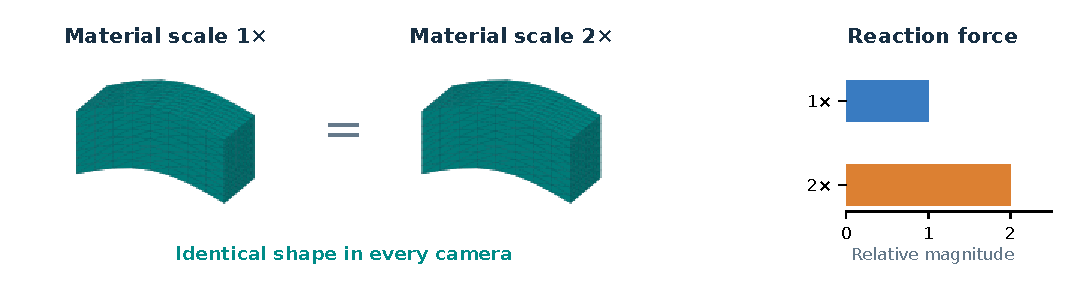
\includegraphics[width=\linewidth]{figures/observability_visual.pdf}
\caption{\textbf{Visual agreement need not identify physical scale.} Co-scaling bulk and attachment energies preserves position-controlled equilibria but changes reactions. An extra view cannot remove this particular ambiguity.}
\label{fig:ambiguity}
\end{figure}

Our numerical counterexample doubles stiffness, obtains a scaled-equilibrium residual of $3.59\times10^{-13}$\,N and produces byte-identical images from all three tested views while doubling reactions. This is a controlled illustration of an exact symmetry, not evidence that all visual inverse problems are unidentifiable. Known gravity or fixed-mass timed dynamics can break this scale symmetry; unknown density can introduce related ambiguities. Breaking one symmetry also does not guarantee globally identifiable parameters.

\paragraph{Actions and uncertainty.}
A new view can reveal previously occluded deformation but cannot reveal a mechanical quantity absent from all geometry. A new action can excite a different strain or attachment regime and reduce prediction error. We test the latter with an extra position observation. We distinguish its empirical benefit from the stronger claim that an uncertainty score selects better actions. In particular, local parameter uncertainty omits model discrepancy and can contract around an inaccurate explanation.

\section{Experiments}
\subsection{Tasks and evaluation protocol}
All experiments are synthetic, with known reference geometry and material correspondences. They isolate mechanics rather than the full image-to-geometry pipeline. We keep four protocols distinct: known-descriptor transfer, unknown-descriptor static refinement, drop forecasting after calibration, and six-family interaction transfer. No cross-task average is reported.

For static tests, coordinate RMSE averages squared errors over points and their three coordinates before taking the square root. In the four-world drop study, dynamic world error is point-vector RMS using reference-area surface weights; shape error additionally removes one best-fitting rigid transform per frame. The latter distinguishes deformation from gross translation and rotation. Vector RMS equals $\sqrt3$ times coordinate RMSE only for identical samples, weights and aggregation without additional alignment.

We retain missing forecasts and distinguish complete-case paired summaries from whole-cohort coverage. Numerical-reference checks separately vary timestep and spatial resolution. An energy or penetration check alone is insufficient to establish spatial convergence. Supplementary material provides solver settings, per-case values, recovery history and videos.

\subsection{Transfer with known descriptors}
Training scenes contain 54 objects and six commands each. Tests comprise six withheld-composition objects and six geometry draws, with four new commands per object and 343 common material queries. The geometry draws use two unseen parameterizations of the same mapped-cuboid topology. All material and attachment descriptors are supplied, so this tests forward transfer rather than inverse identification. Predictions use resolution $n=4$ and analytic references $n=8$; the structured element layout is $(4n,n,n)$.

We compare shared laws with a matched analytic teacher, a Neo-Hookean alternative, and custom DeepSets direct predictors trained for 6,000 or 30,000 steps on the same 324 scene responses. These are supervised controls, not published graph-network baselines. The direct predictors receive matched descriptors and frozen-law fingerprints. Their reported stable controls repair zero-variance input normalization with physical units while keeping weights fixed; the supplement records the original failures and recovery protocol.

\begin{table}[t]
\centering\small
\caption{\textbf{Known-descriptor forward transfer.} Coordinate RMSE in mm; six objects and four commands per object in each column. Direct is a custom 30k-step stable normalization control.}
\label{tab:transfer}
\begin{tabular}{lrr}\toprule
Method & Compositions & Geometries\\\midrule
Matched analytic & 0.0164 & 0.0159\\
Shared laws & 0.0181 & 0.0183\\
Custom direct, 30k & 3.0888 & 3.2933\\\bottomrule
\end{tabular}
\end{table}

Table~\ref{tab:transfer} shows that shared local laws remain close to the matched analytic model under these changes, while the direct predictor has larger errors. Figure~\ref{fig:transfer} includes both training budgets and the simpler constitutive control. This supports reuse within the represented law family; it does not establish transfer to arbitrary unseen materials or interaction types. The small analytic-model error also includes discretization differences.

\begin{figure*}[t]
\centering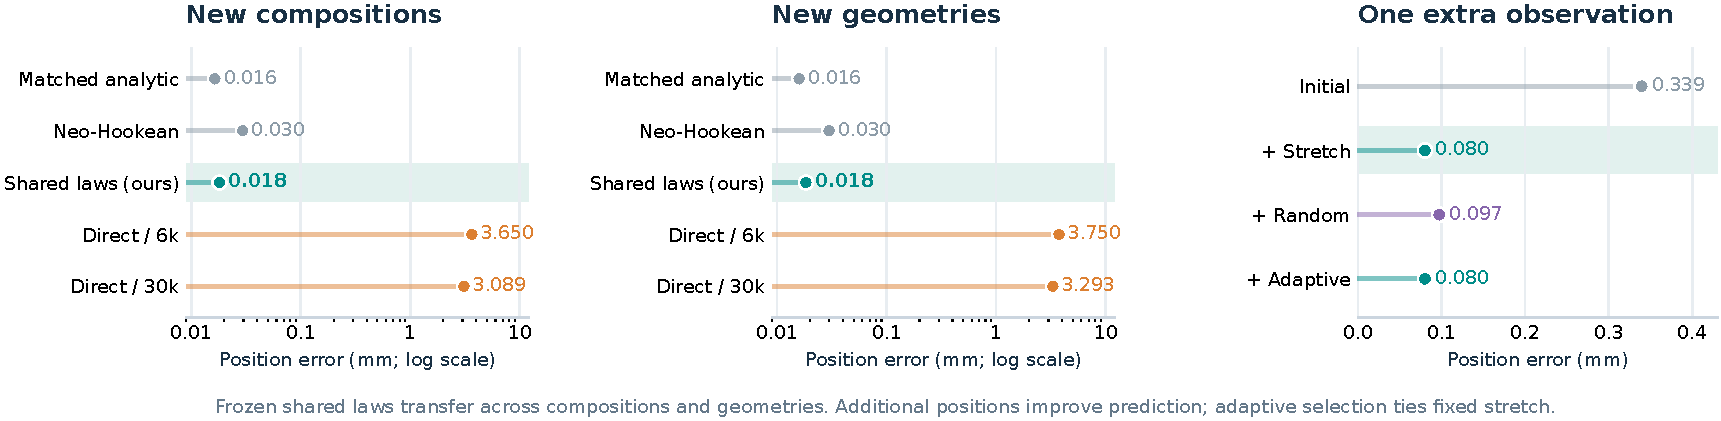
\includegraphics[width=\textwidth]{figures/transfer_visual.pdf}
\caption{\textbf{Forward transfer and additional observations.} Left and center: known-descriptor coordinate RMSE for new compositions and geometry draws, on logarithmic axes. Right: unknown-descriptor prediction error after one additional observation. Adaptive selection chooses the same stretch on every object and ties the fixed stretch policy. Direct controls use frozen weights with the documented stable normalization.}
\label{fig:transfer}
\end{figure*}

\subsection{Refining unknown descriptors with an action}
A separate experiment uses six fresh objects, 26 observed/scored points, 50\,$\mu$m position noise and two withheld commands per object. Geometry, categorical material/interface families, heterogeneity pattern, gravity and density are known; 15 continuous descriptors are fitted. Inference uses $n=2$ and the analytic reference $n=4$. No reactions are observed.

An extra stretch observation lowers mean held-command position coordinate RMSE from 0.3395 to 0.0802\,mm and reaction coordinate RMSE from 0.0961 to 0.0292\,N. Thus position observations can improve predictions of an unobserved physical output when the setup provides an independent scale. The variance-based policy selects stretch for all six objects, however, and exactly ties the fixed stretch policy. It has no demonstrated advantage over that strong fixed choice. Of 48 fits across the declared variants, 41 converge and seven incomplete fits are retained; all stretch fits converge.

Moreover, nominal 90\% position-interval coverage falls from 97.0\% initially to 33.0\% after stretch. Better point predictions coexist with worse uncertainty calibration. We therefore report the additional-observation result as prediction refinement, not as calibrated active system identification.

\subsection{Dynamic prediction against native PhysTwin}
The fresh cohort has four worlds: two Mooney--Rivlin and two Yeoh-type materials with randomized scale, shape and contact stiffness. Each uses a $12\!\times\!6\!\times\!6$\,cm block of mass 0.27\,kg under gravity. Calibration observes a 10\,mm drop for 0.20\,s; forecasts predict 40 and 80\,mm drops for 0.30\,s at 100\,Hz. This is an out-of-calibration load-amplitude test within the same contact class, not unknown-interaction-type generalization. Calibration uses noiseless visible 3D tracks. Ninety-eight unique surface points and reference-area weights are shared for scoring.

We run the authors' native PhysTwin implementation~\cite{jiang2025phystwin}, retaining its 125-node spring graph and native fitting pipeline. A global recipe of at most 100 CMA generations, retaining native early stopping, and 1,000 optimization epochs is chosen on development calibration only and frozen before fresh world draws. Our continuum model uses $n=3$ and 50\,$\mu$s timesteps; the primary reference uses $n=4$ and 25\,$\mu$s. Native and continuum parameterizations, mass distributions, damping and contact models differ, so this is a configuration-level comparison rather than an isolated architecture ablation.

Our method completes all eight forecasts. Native PhysTwin completes six; one world's graph initialization fails with an empty graph before its two forecasts. These are recorded as unavailable, not zero error or omitted successes. On the paired six forecasts from three worlds, world-space vector RMS is 1.146 versus 13.771\,mm and rigid-aligned shape RMS is 1.085 versus 2.936\,mm (Table~\ref{tab:dynamic}). The world-space gap is substantially larger than the shape gap, demonstrating why rigid-aligned scoring matters.

\begin{table}[t]
\centering\small
\caption{\textbf{Fresh dynamic cohort.} Error means condition on the six forecasts available to both methods. No complete eight-forecast paired mean exists. Held-view means use the same three worlds.}
\label{tab:dynamic}
\begin{tabular}{lrr}\toprule
Measure & Ours & Native PhysTwin\\\midrule
Forecasts completed & 8/8 & 6/8\\
World vector RMS (mm)$\downarrow$ & 1.146 & 13.771\\
Shape vector RMS (mm)$\downarrow$ & 1.085 & 2.936\\
Centroid error (mm)$\downarrow$ & 0.346 & 13.412\\\midrule
Held FG PSNR (dB)$\uparrow$ & 18.73 & 12.84\\
Held FG SSIM$\uparrow$ & 0.747 & 0.577\\
Held silhouette IoU$\uparrow$ & 0.956 & 0.795\\
Visible depth error (mm)$\downarrow$ & 5.478 & 14.557\\\bottomrule
\end{tabular}
\end{table}

\begin{figure*}[t]
\centering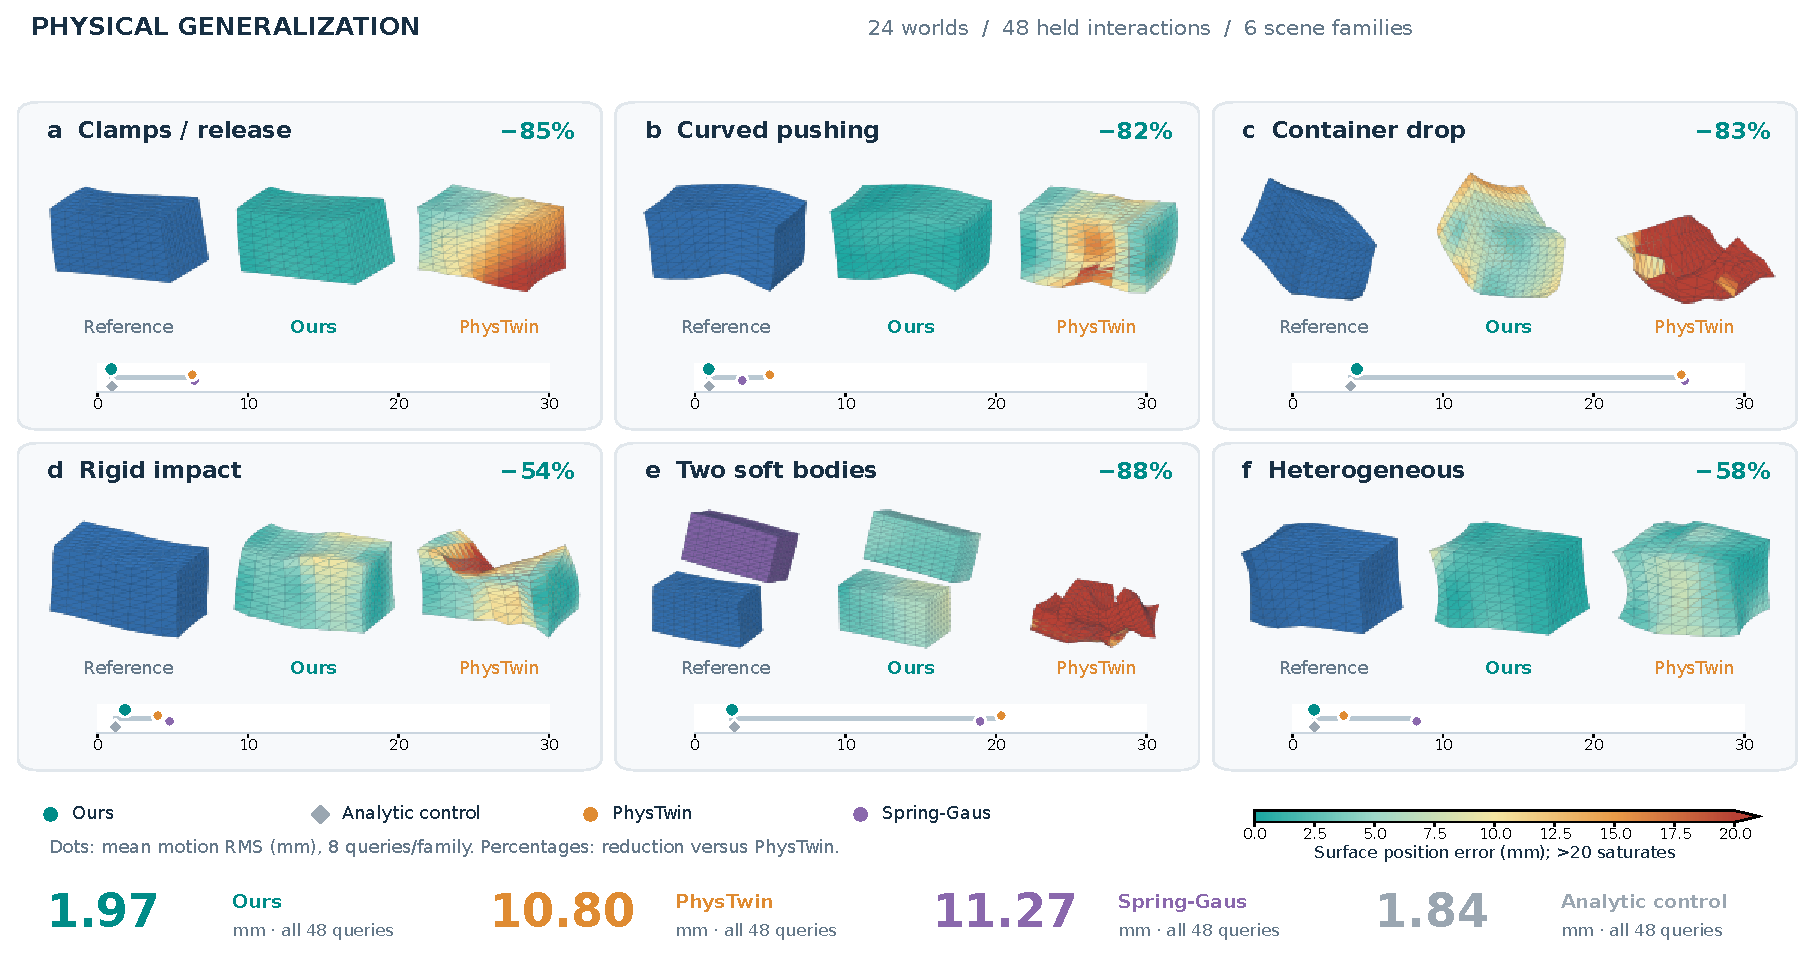
\includegraphics[width=.96\textwidth]{figures/held_visual_results.pdf}
\caption{\textbf{Physical prediction across six interaction families.} Each panel shows the first world, query 0, final frame; error colors share a 0--20\,mm scale. Dots use all eight queries per family; percentages report mean-error reduction versus PhysTwin. The footer reports all 48 queries. Ours has lower mean error than both native spring adaptations in every family; the analytic control remains competitive. The supplement shows every comparator and the earlier drop cohort.}
\label{fig:held-visual}
\end{figure*}

\paragraph{Appearance under predicted dynamics.}
Both models use the same initial appearance checkpoint, with 10,059 surviving Gaussians after training on three initial views. We freeze appearance and evaluate three observed and two withheld cameras over all 31 forecast frames. There are 2,480 method/image slots: 2,170 scored and 310 unavailable native slots. The paired held-view comparison uses 372 of 496 possible images per method, averaged equally over the same three worlds. Initial rendered RGB is byte-identical for paired queries. Held-view foreground PSNR and SSIM favor our model (Table~\ref{tab:dynamic}), while the supplement illustrates the first declared world's 80\,mm forecast. These results concern physical trajectories and different transport rules with shared appearance, not superior radiance reconstruction.



\paragraph{Reference and optimizer sensitivity.}
All 20 reference-check simulations complete and pass individual energy, Jacobian and penetration checks. All four timestep comparisons pass, but all four declared spatial comparisons fail. In a post-hoc subset of two 80\,mm forecasts, changing the reference from $n=4$ to $n=6$ changes our world errors from 1.180 to 1.690\,mm and from 1.485 to 1.660\,mm; the native errors change from 19.424 to 18.779\,mm and from 17.720 to 17.005\,mm. A further half timestep has little effect, and the ordering remains unchanged. This supports the ordering on this subset but does not qualify the primary reference as spatially converged. Predictions are not refitted to the refined targets.

Only one of 16 final dynamic optimizer searches meets its convergence criterion; 15 exhaust their declared budgets. Forecast coverage therefore measures saved finite trajectories, not certainty that the best physical parameters were recovered. A development-only removal of fitted native damping reduces world error from 9.518 to 6.147\,mm while worsening shape error from 2.304 to 2.761\,mm. Damping explains part of the gap, and our conservative prior matches the conservative teacher. Native graph mass discretization also changes rest inertia. These controls limit a claim of architecture-only superiority.

\subsection{Stronger deformation and contact examples}
The accompanying examples extend beyond barely visible motion. Prescribed 30\% tool closure produces 22.7\% material shortening; six mesh, timestep and quadrature configurations qualify that compression cycle. A finite 80\,g sphere of radius 25\,mm striking at 1\,m/s produces 13.6\% central compression and rebound. A separate viscous 40\,mm drop demonstrates bounce and settling over 0.75\,s. The impact and viscous examples are demonstrations, not spatially qualified comparative inference results. Abrupt-release failures at stronger deformation are retained. These examples demonstrate supported interactions beyond the quantitative forecast cohort.

\subsection{Six-family interaction transfer}
We extend the comparison to movable/released clamps, curved-obstacle
pushing, drops into containers and obstacles, finite-mass rigid strikers,
two interacting deformable objects, and heterogeneous material. A frozen
protocol draws four independent material worlds per family. Each method
fits one short position-track prefix, seals its parameters, and predicts
two changed interactions without refitting: 24 worlds and 48 queries.
Geometry, mass and boundary recipes are supplied; materials are unknown.
This study tests changes within explicit interaction families, not discovery
of arbitrary unknown contact laws. A development-selected extension of our
bulk energy adds an independently fitted volumetric coefficient and
per-body/spatial material descriptors; prior-study results are preserved.

Figure~\ref{fig:held-visual} and Table~\ref{tab:complex-main} compare native PhysTwin and Spring-Gaus
adaptations, our model and a fitted analytic control with knowledge of the
reference constitutive family. Every method uses the declared common
observations and queries; native spring parameterizations and fitting
budgets differ from continuum parameterizations. UniPhy is evaluated on
eight supported drop queries: one completes and seven fail with native CFL
errors; 40 other slots are unsupported by this adapter. No complete
paired world exists for UniPhy. The supplement specifies implementations,
budgets, coverage and development controls.

\begin{table}[t]
\centering\small\setlength{\tabcolsep}{4pt}
\caption{\textbf{Six-family held interaction transfer.} All listed methods
complete 48 queries. Physical vector RMS is in mm. Foreground PSNR uses
shared Gaussian appearance and transport, averaged over noninitial query
frames. This is not native end-to-end reconstruction quality.}
\label{tab:complex-main}
\begin{tabular}{lrrr}
\toprule Method & Motion & Shape & FG PSNR \\
\midrule
\textcolor{oursteal}{\textbf{Ours}} & \textbf{1.97} & \textbf{1.25} & \textbf{35.61} \\
Analytic control & 1.84 & 1.16 & 36.02 \\
PhysTwin adaptation & 10.80 & 5.94 & 25.68 \\
Spring-Gaus adaptation & 11.27 & 6.00 & 25.88 \\
\bottomrule
\end{tabular}
\end{table}

Our paired motion-error difference is $-8.83$\,mm against PhysTwin
(world-bootstrap 95\% interval $[-12.18,-5.83]$) and $-9.30$\,mm
against Spring-Gaus ($[-12.40,-6.50]$). Ours has lower mean motion
error in each family than either native adaptation. Against the analytic
control, the difference is $+0.13$\,mm ($[-0.01,0.27]$), so an
advantage over that control is not established. Common sampled material-grid
inversions occur in 0/48 queries for ours and analytic, 33/48 for PhysTwin
and 37/48 for Spring-Gaus; these diagnostics do not certify continuous
validity. Eleven of twelve refinement comparisons complete;
the stacking run times out (supplement). The shared-renderer scores measure the image consequences of
predicted motion independently of appearance optimization.


\section{Discussion and Limitations}
The strongest supported result is that reusable local laws can predict held responses accurately within a controlled family, and can improve physical trajectories and rendered forecasts relative to configured native adaptations in controlled synthetic cohorts. The scale example explains why images and physics must be evaluated separately. Additional observations help point prediction, but our uncertainty model and action selection do not yet justify reliable autonomous probing.

The experiments supply geometry, correspondences, density and substantial family knowledge. They do not establish image-only identification, performance on real captures, arbitrary unknown boundary conditions, or frictional multi-object contact. Constitutive teachers overlap the modeled family. The earlier drop study has four worlds, and the six-family study has four worlds per family. Its forecasts are correlated within worlds; we do not treat hundreds of rendered frames as independent physical trials. The earlier native baseline has two missing forecasts; UniPhy has limited coverage in the six-family study. Native adaptations differ in important physical priors. Reference spatial convergence remains unresolved for the main drop cohort.

Further evaluation should add independent material families, real observations, matched dissipative assumptions, and spatially qualified references. For active identification, views should reveal uncertain geometry and interactions should distinguish physical responses. Calibrated action selection remains open.

\section{Conclusion}
Our compositional representation separates shared bulk and attachment laws from loads, contact and appearance. Frozen constitutive decoders support position-driven prediction and scene-specific fitting. Transfer, refinement and dynamic experiments show prediction gains while exposing limits of visual agreement, local uncertainty and finite-resolution references. Digital twins must be judged by withheld physical responses as well as rendered images.

\clearpage
\section*{LLM Usage Statement}
OpenAI Codex was used extensively to assist with implementation, experiment orchestration, literature discovery, analysis checks, manuscript drafting and programmatic figure generation. Numerical results are drawn from saved experiment artifacts; scientific figures and qualitative panels are generated from those artifacts rather than synthesized as experimental evidence. This assistance does not replace author responsibility for validating the methods, references, results and final submission.
{\small\bibliographystyle{ieeenat_fullname}\bibliography{references}}
\end{document}
